\subsection{Modify an existing task}

It may happen that the user wants to modify an existing task since his travel mean preferences are changed or the appointment time or location are changed. It can also be the case that the user wants to delete a scheduled appointment. These features are described in this section. Notice that, an overlap may occur caused by the task modification, in this case the System will handle the situation as described in the Add a FixedTask Use Case.

\begin{table}[H]
	\centering
    
    \begin{tabular}{|p{3.5cm}|p{10.3cm}|}
    
    \hline
    \textbf{\large{Actors}}  			& \tabitem User\\
    
    \hline
    \textbf{\large{Goals}} 				& \ref{goal:task}; \ref{goal:taskBehavior}; \ref{goal:impossibleTask}; \ref{goal:preferences}; \ref{goal:retakeCar}\\
    
    \hline
    \textbf{\large{Enter Condition}}	& The user should be logged in the                                                        \emph{Travlendar+} System\\
    
    \hline
    \textbf{\large{Events Flow}}		& \begin{enumerate}[leftmargin=0.5cm]
                                             
                                          	\item The user select the task he wants to change from his calendar (doing this he can also change the time scope of the calendar: daily, weekly, monthly time scope)
                                          	\item Now he can decide to modify some preferences, such as the time, the date, the location or the priority of the selected task. Moreover, the user can choose to cancel the entire task
                                          	\item The user confirm to apply the changes or discard them
                                          	\item The \emph{Travlendar+} System computes a new schedule according to the new user preferences
                                          	\item Finally the user can choose from the new calendar or the older one
                                          \end{enumerate}
    										\\
    \hline
    \textbf{\large{Exit Condition}} 	& The user has chosen which calendar he prefers:                                          the newer or the older; So, from now on, the System will behave accordingly to the updated calendar\\
    
    \hline
    \textbf{\large{Exception}} 			& The modification of the task is not valid, for instance the user has inserted some wrong information about the task, then the user has to modify the task again. \newline
    The modification of the task has created an overlap with another task, so the user has to choose which task he prefers to have in his calendar.\\
    
    \hline
    
    
    \end{tabular}
	
\end{table}

\begin{figure}[H]
\centering
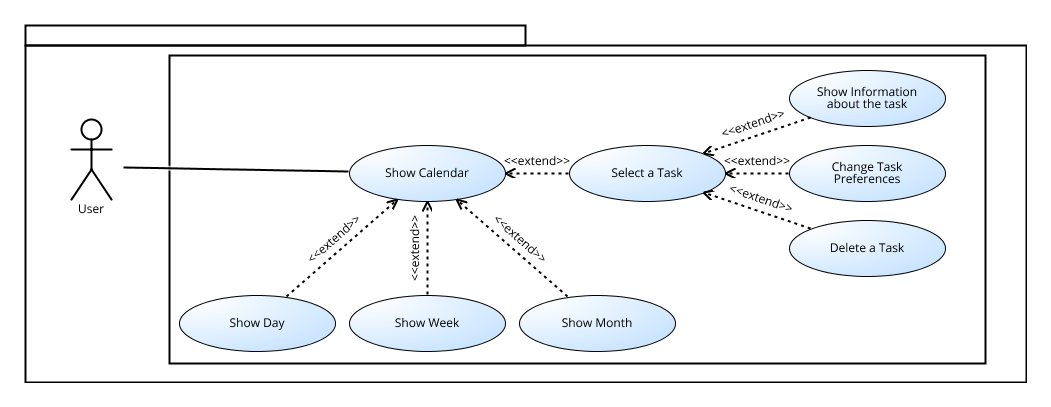
\includegraphics[scale=0.5]{Pictures/UseCaseDiagram/Rescheduling.png}
\caption{UML Use Case Diagram for the modification of a new task and the rescheduling of the calendar}
\end{figure}

\begin{figure}[H]
\centering
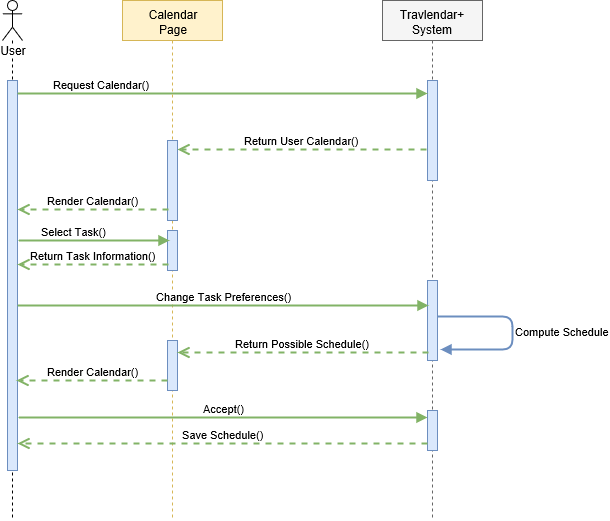
\includegraphics[scale=0.5]{Pictures/SequenceDiagram/rescheduling.png}
\caption{UML Sequence for the modification of a new task and the rescheduling of the calendar}
\end{figure}